\section{Self-Supervised Learning: Wav2Vec 2.0}

\begin{frame}[plain]
  \centering
  \vspace{0.10\textheight}
  {\LARGE \textbf{Self-Supervised Learning: Wav2Vec 2.0}}

  \vspace{0.08\textheight}
  {\large Learning speech representations from unlabeled audio}
\end{frame}

\begin{frame}[allowframebreaks]{Wav2Vec 2.0: Overview}
    \begin{itemize}
        \item \textbf{Proposed by Baevski et al. (2020)}
        \item \textbf{Key Idea:} Self-supervised learning for speech representation.
        \item \textbf{Architecture:}
        \begin{itemize}
            \item CNN encoder for raw waveform $\rightarrow$ latent representations $z_t$
            \item Transformer for context representations $c_t$
            \item Quantization module for discrete representations $q_t$
        \end{itemize}
    \end{itemize}
    \begin{figure}[h]
        \centering
        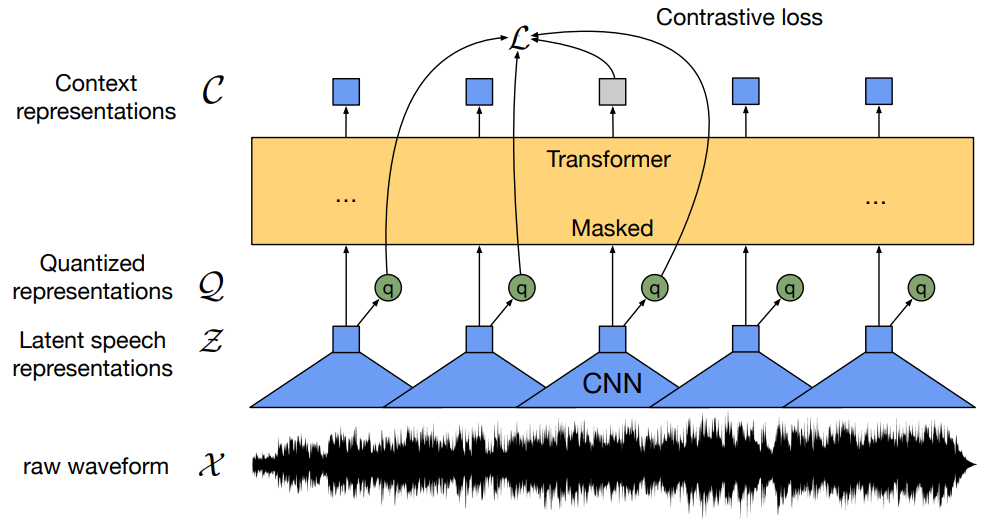
\includegraphics[width=\textwidth,height=0.72\textheight,keepaspectratio]{images/audio-nlp/wav2vec2-overview.png}
        \caption*{Wav2Vec 2.0 architecture overview.}
    \end{figure}
    \slideimgsource{Baevski et al., wav2vec 2.0, Fig.~1; \href{https://arxiv.org/abs/2006.11477}{arXiv:2006.11477}.}
\end{frame}

\begin{frame}{Wav2Vec 2.0: Feature Extraction}
    \begin{itemize}
        \item \textbf{Step 1:} Raw audio waveform is input to a multi-layer CNN encoder.
        \item \textbf{Output:} Latent speech representations $z_t$.
    \end{itemize}
    \begin{center}
        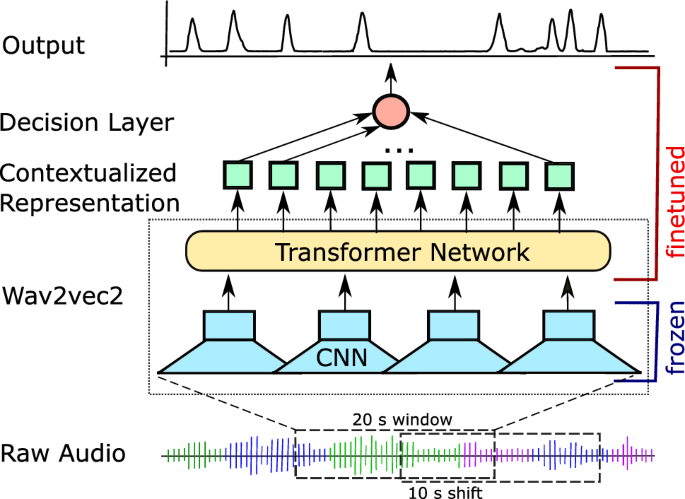
\includegraphics[width=\textwidth,height=0.46\textheight,keepaspectratio]{images/audio-nlp/wav2vec2-cnn.png}
    \end{center}
    \[
        \text{Waveform} \xrightarrow{\text{CNN}} z_t
    \]
    \slideimgsource{Kune\v{s}ov\'a et al., ``Comparison of wav2vec 2.0 models on three speech processing tasks,'' \textit{Int.\ J.\ Speech Technology} 27(4):847--859, 2024, Fig.~2; \href{https://doi.org/10.1007/s10772-024-10140-6}{doi:10.1007/s10772-024-10140-6}. Shown there as a fine-tuned frame classifier, not as the wav2vec 2.0 pre-training model.}
\end{frame}

\begin{frame}{Wav2Vec 2.0: Contextualization and Masking}
    \begin{itemize}
        \item \textbf{Step 2:} Random spans of $z_t$ are masked.
        \item \textbf{Step 3:} Transformer network produces contextualized representations $c_t$.
    \end{itemize}
    \[
        z_t \xrightarrow{\text{mask spans}} \xrightarrow{\text{Transformer}} c_t
    \]
\end{frame}

\begin{frame}{Wav2Vec 2.0: Quantization}
    \begin{itemize}
        \item \textbf{Step 4:} Quantize $z_t$ to discrete representations $q_t$.
        \item \textbf{Quantization:} Product of $G$ codebooks, each of size $V$.
    \end{itemize}
    \[
        z_t \xrightarrow{\text{Quantization}} q_t
    \]
\end{frame}

\begin{frame}{Wav2Vec 2.0: Contrastive and Diversity Losses}
    \begin{itemize}\footnotesize
        \item \textbf{Contrastive loss.} At each masked step, identify the true quantized latent $q_t$ within a candidate set $Q_t$ holding $q_t$ itself plus $K = 100$ distractors sampled from other masked steps of the same utterance.
    \end{itemize}
    \[
        \mathcal{L}_m = -\log \frac{\exp\!\big(\mathrm{sim}(c_t, q_t) / \kappa\big)}
                                   {\sum_{\tilde{q} \in Q_t} \exp\!\big(\mathrm{sim}(c_t, \tilde{q}) / \kappa\big)}
    \]
    \begin{itemize}\footnotesize
        \item $\mathrm{sim}$ is cosine similarity and $\kappa = 0.1$ is a temperature. The sum runs over \emph{all} of $Q_t$, the positive included, so the ratio is a softmax over candidates.
        \item \textbf{Diversity loss} $\mathcal{L}_d$ encourages use of every codebook entry, stopping the quantizer collapsing onto a handful of codes. Total objective: $\mathcal{L} = \mathcal{L}_m + \alpha \mathcal{L}_d$.
    \end{itemize}
    \slideimgsource{Baevski et al., wav2vec 2.0, Eq.~3; \href{https://arxiv.org/abs/2006.11477}{arXiv:2006.11477}.}
\end{frame}

\begin{frame}{Wav2Vec 2.0: Performance}
    \begin{itemize}\footnotesize
        \item LibriSpeech \textbf{test-clean} WER, LARGE model pre-trained on 53.2k hours of unlabeled LibriVox audio and decoded with a Transformer LM:
        \begin{itemize}
            \item 1.8\% fine-tuned on the full 960 h of labeled data (3.3\% on test-other)
            \item 4.8\% fine-tuned on only 10 minutes of labeled data (8.2\% on test-other)
        \end{itemize}
        \item \textbf{The language model is doing real work.} Strip it out and that same 10-minute model lands near 40\% WER. Always quote self-supervised numbers with the decoding setup attached.
        \item \textbf{Impact:} makes unlabeled audio usable, which matters most where labeled speech is scarce.
    \end{itemize}
    \begin{center}
        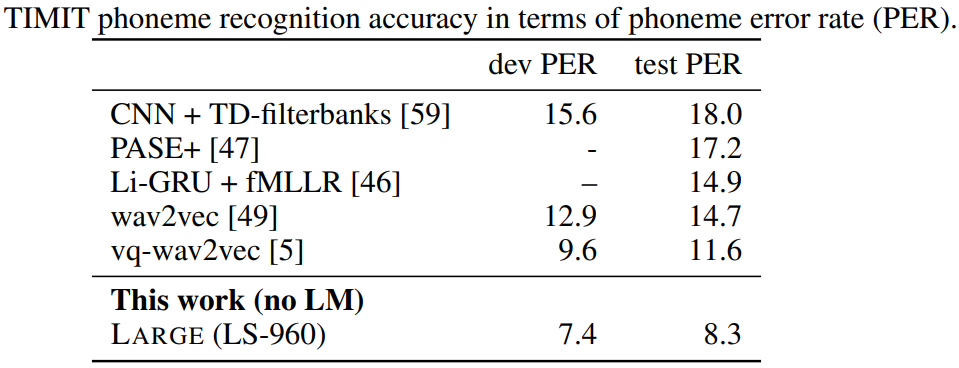
\includegraphics[width=0.44\textwidth]{images/audio-nlp/wav2vec2-results.png}
    \end{center}
    \slideimgsource{Baevski et al., wav2vec 2.0: the WERs above are LibriSpeech (Tables~1, 2 and 9); the table shown is Table~3, a \emph{separate} TIMIT phoneme-error-rate benchmark decoded without an LM. \href{https://arxiv.org/abs/2006.11477}{arXiv:2006.11477}.}
\end{frame}
